\documentclass[12pt]{article}
\usepackage[a4paper, hmargin={2.5cm, 2.5cm}, vmargin={2.5cm, 2.5cm}]{geometry}

\usepackage[nottoc,numbib]{tocbibind}

\usepackage[utf8]{inputenc}
\usepackage[english]{babel}
\usepackage{amssymb}
\usepackage{amsfonts}
\usepackage{amsmath}
\usepackage{setspace}
\usepackage{algorithm}
\usepackage[noend]{algpseudocode}

\usepackage{tikz}
\usetikzlibrary{positioning,shapes, shadows, arrows, automata}

\usepackage{xcolor}
\usepackage{listings}
\usepackage{graphicx}
\usepackage[hidelinks]{hyperref}
\usepackage{float}
\usepackage[english]{varioref}
\usepackage{multirow}
\usepackage{hhline}
\usepackage{etoolbox}
\usepackage{seqsplit}

\usepackage{fancyhdr}

\setlength\parindent{0pt}
\usepackage[parfill]{parskip}

\definecolor{pblue}{rgb}{0.13,0.13,1}
\definecolor{pgreen}{rgb}{0,0.5,0}
\definecolor{pred}{rgb}{0.9,0,0}
\definecolor{pgrey}{rgb}{0.46,0.45,0.48}

\definecolor{mygray}{rgb}{0.9451,0.9451,0.9451}

\lstset{
  language=Java,
  backgroundcolor=\color{mygray},
  basicstyle=\footnotesize\ttfamily,
  commentstyle=\color{pgreen},
  keywordstyle=\color{pblue},
  stringstyle=\color{pred},
  mathescape,
  breaklines=true,
  numbers=left,
  numberstyle=\ttfamily,
  stepnumber=1,
  firstnumber=1,
  numberfirstline=true,
  postbreak=\raisebox{0ex}[0ex][0ex]{\ensuremath{\color{red}\hookrightarrow\space}},
  literate={->}{$\rightarrow$}{2}
           {ε}{$\varepsilon$}{1}
}

\linespread{1.3}

\title{
  \vspace{4cm}
  \begin{flushleft}
  \Large{\textbf{Theory Assignment}} \\
  \large{Artificial Intelligence and Multi Agent Systems}
  \end{flushleft}
  \vspace{0cm}
  \begin{flushleft}
  \small
  \textit{\today}
  \end{flushleft}
  \vspace{12cm}
  \begin{flushleft}
  \small
  Troels Thomsen \texttt{s152165} \\
  Rasmus Haarslev \texttt{s152175} \\
  \end{flushleft}
}

\date{
	%
}

\begin{document}

\clearpage
\pagenumbering{gobble}
\thispagestyle{empty}
\maketitle

\newpage

\section*{Exercise 1}

\subsection*{a)}
\label{sub:a)}

\textit{DipBrush} If we assume that cans contain colours, we can omit the IsColor literal since we can infer that $k$ must be a color of it is in a can.

\textit{Paint} The same argument for removing the IsColor literal from \textit{DipBrush} can be repeated for \textit{Paint}. We can remove the Brush literal from \textit{Paint}, since CanPaint is an effect of \textit{DipBrush}, which has the Brush literal as a precondition.

\subsection*{b)}
\label{sub:b)}

$\neg CanPaint(r, k)$ denotes that the brush no longer contains a color. The robot keeps painting with the same brush until it runs out of color and has to $DipBrush$ again.

\subsection*{c)}
\label{sub:c)}

$Block(b)$, $Brush(r)$, and $Can(c)$ are the rigid atoms in this planning domain.

\subsection*{d)}
\label{sub:d)}

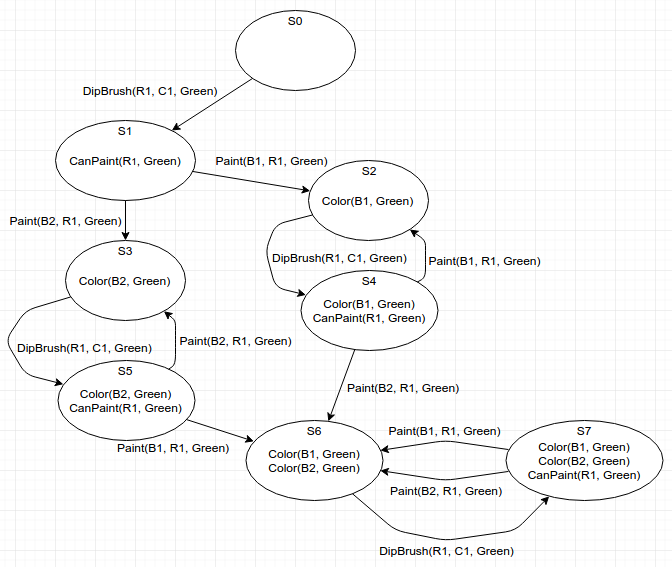
\includegraphics[scale=0.6]{statespace.png}

\subsection*{e)}
\label{sub:e)}

\begin{enumerate}
    \item DipBrush(R1, C1, Green)
    \item Paint(B1, Green)
    \item DipBrush(R1, C1, Green)
    \item Paint(B2, Green)
\end{enumerate}

\end{document}
